\subsection{Written by me} \vspace{-.1in}
\subsubsection{Week 2 | Exercise 2.23} \vspace{-.05in}

This is Exercise 2.23 from Week 2.
This was with Daniel and Kirat. Part of the write-up is by Daniel.

\begin{exr}[num=2.23]
    Let $ (X, d_{X}), (Y, d_{Y}) $ be metric spaces,
    and $ A \subseteq X, B \subseteq Y $ subsets.
    Then, $ \overline{A \times B} = \overline{A} \times \overline{B} $.
\end{exr}

\begin{pf}[source=Daniel]
    First, we show that $ \overline{A \times B} \subseteq \overline{A} \times
    \overline{B} $. \vsp
    %
    Let $ (a, b) \in \overline{A \times B} $ be given.
    We must show that $ (a, b) \in \overline{A} \times \overline{B} $,
    for which it suffices to prove that given any $ \varepsilon > 0 $,
    the sets $ B_{\varepsilon}(a) \cap A $ and $ B_{\varepsilon}(b) \cap B $ are
    non-empty. \vsp
    %
    Let $ \varepsilon > 0 $ be given.
    Take $ (p, q) \in B_{\varepsilon}((a,b)) \cap (A \times B) $. \\
    Then we have that:
    \begin{equation*}
        d_{X \times Y}((a,b), (p,q)) = d_X(a, p) + d_Y(b, q) < \varepsilon
    \end{equation*}
    Rearranging, and using non-negativity of distance functions we get that:
    \begin{align*}
        & d_X(a, p) < \varepsilon - d_Y(b, q) \\
        \implies \ & d_X(a, p) < \varepsilon \\
        & d_Y(b, q) < \varepsilon - d_X(a, p) \\
        \implies \ & d_Y(b, q) < \varepsilon
    \end{align*}
    from which it follows that $p\in B_{\varepsilon}(a)\cap A$ and $q\in
    B_{\varepsilon}(b)\cap B$.
\end{pf}

\begin{pf}[source=Me]
    Next, we show that $ \overline{A} \times \overline{B} \subseteq
    \bar{A \times B} $. \npgh
    
    Let $ (a, b) \in \bar{A} \times \bar{B} $.
    Then, for all $ \ep > 0 $, we have that $ B(a, \frac{\ep}{2}) \cap A \neq
    \varnothing $, and $ B(b, \frac{\ep}{2}) \cap B \neq \varnothing $.
    We want to show that $ (a, b) \in \bar{A \times B} $. \vsp
    %
    To do this, choose $ p \in B(a, \frac{\ep}{2}), q \in B(b, \frac{\ep}{2}) $.
    We see that:
    \begin{align*}
        & d_{X \times Y}((a, b), (p, q)) \\
        = \ & d_{X}(a, p) + d_{Y}(b, q) \\
        < \ & \frac{\ep}{2} + \frac{\ep}{2} \\
        = \ & \ep
    \end{align*}
    Therefore, we have that $ (p, q) \in B((a, b), \ep) $.
    Since this is true for all $ \ep > 0 $, we therefore conclude that
    $ B_{\ep}(a, b) \cap A \times B \neq \varnothing $ for all $ \ep > 0 $.
    Therefore, $ (a, b) \in \bar{A \times B} $ as needed.
\end{pf}

\newpage
\subsubsection{Week 4 | Exercise 4.11}
The following is Exercise 4.11 from Week 4.
This was solved and written independently.

\begin{exr}[num=4.11]
    Let $ (X, d_{X}) $ and $ (Y, d_{Y}) $ be two metric spaces, and let
    $ f: X \rightarrow Y $ be a function such that for any open subset $ U
    \subseteq Y $, we have that $ f^{-1}(U) $ is an open subset of $ X $. \vsp
    %
    Let $ (x_{n})_{n \geq 1} $ be a sequence in $ X $ such that $ x_{n}
    \rightarrow x_{0} $. Prove that $ f(x_{n}) \rightarrow f(x_{0}) $.
\end{exr}

\begin{pf}
    Suppose $ (x_{n})_{n \geq 1} $ is a sequence such that $ x_{n} \rightarrow
    x_{0} $ for some $ x_{0} \in X $. \vsp
    %
    Consider $ B = B(f(x_{0}), r) $ for some $ r > 0 $.
    Note that since $ f(x_{0}) \in B $, we clearly have $ f^{-1}(f(x_{0})) =
    x_{0} \in f^{-1}(B) $. Since $ B $ is an open set in $ Y $, then
    $ f^{-1}(B) $ is also an open set in $ X $. \vsp
    %
    Since $ f^{-1}(B) $ is open, then there exists some $ \delta > 0 $ such that
    $ B(x_{0}, \delta) \subseteq f^{-1}(B) $.
    Additionally, since $ x_{n} \rightarrow x_{0} $, then for all $ \ep > 0 $,
    there exists some $ N \geq 1 $ such that for all $ i \geq N, d_{X}(x_{i},
    x_{0}) < \ep $. In particular, fix $ \ep_{0} < \delta $ to be any such value.
    However, since each such $ x_{i} \in B(x_{0}, \ep_{0}) $, it follows that:
    \begin{equation*}
        x_{i} \in B(x_{0}, \ep_{0}) \subseteq B(x_{0}, \delta) \subseteq
        f^{-1}(B)
    \end{equation*}
    Since each $ x_{i} \in f^{-1}(B) $, then $ f(x_{i}) \in B $.
    That is, there is a tail of the sequence $ f(x_{n}) $ such that
    each $ f(x_{i}) \in B = B(f(x_{0}), r) $.
    But since this is true for all $ r > 0 $, then this precisely means that for
    all $ \ep > 0 $, there exists some $ M \geq 1 $ such that for all $ i
    \geq M $, $ d_{Y}(f(x_{i}), f(x_{o})) < \ep $. \vsp
    %
    Therefore, we see that $ f(x_{n}) \rightarrow f(x_{0}) $ as required.
\end{pf}

\newpage
\subsubsection{Week 6 | Exercise 6.31(i)}

The following is Exercise 6.31(i) from Week 6.
This was solved and written independently.

\begin{exr}[num=6.31(i)]
    Let $ (X, d) $ be a metric space.
    Prove that if $ d $ is topologically equivalent to the discrete metric,
    then $ (X, d) $ has no infinite compact subsets.
\end{exr}

\begin{pf}
    Suppose $ d \sim d_{\trm{disc}} $.
    Note that this implies that every subset is open; in particular, singleton
    sets are open. \vsp
    %
    Let $ A \subseteq X $ be an infinite subset. We can write $ A $ as:
    \begin{equation*}
        A \ = \ \bigcup_{x \in A} \set{x}
    \end{equation*}
    In particular, since each singleton set is open, then this is an open cover
    of $ A $. However, it clearly has no finite subcover, so $ A $ cannot be
    compact. \vsp
    %
    Since this holds true for any infinite subset, then $ X $ has no infinite
    compact subsets.
\end{pf}

\newpage
\subsubsection{Week 8 | Exercise 6.39}

The following is Exercise 6.39 from Week 8.
This was solved together with Alan, and part of the write-up is done by Alan.

\begin{exr}[num=6.39]
    Prove that $ \norm{\cdot} \sim \norm{\cdot}' $ if and only if
    $ \norm{\cdot} \approx \norm{\cdot}' $.
\end{exr}

\begin{pf}[source=Me]
    Suppose $ \norm{\cdot} \sim \norm{\cdot}' $. Consider the identity map
    defined as:
    \begin{gather*}
        I : (X, \norm{\cdot}) \rightarrow (X, \norm{\cdot}') \\
        I^{-1} : (X, \norm{\cdot}') \rightarrow (X, \norm{\cdot})
    \end{gather*}
    Since $ \norm{\cdot} \sim \norm{\cdot}' $, it follows that $ I, I^{-1} $ are
    topologically continous, and thus continuous. Since they are also trivially
    linear, they are therefore bounded. Then, there exist $ m, M \geq 0 $ such
    that:
    \begin{gather*}
        \norm{I(x)}' = \norm{x}' \leq m \norm{x} \\
        \norm{I^{-1}(x)} = \norm{x} \leq M \norm{x}'
    \end{gather*}
    Note that if either $ m $ or $ M $ is equal to $ 0 $, then both norms are the
    $ 0 $ function. Otherwise, we see that:
    \begin{equation*}
        \frac{1}{M}\norm{x} \leq \norm{x}' \leq m\norm{x}
    \end{equation*}
    So we have that $ \norm{\cdot} \approx \norm{\cdot}' $ as needed.
\end{pf}

\newpage
\begin{pf}[source=Alan]
    For the converse, suppose $\Vert \cdot \Vert \approx \Vert \cdot
    \Vert^\prime$. This means there exists $\alpha > 0$ and $\beta > 0$ such that
    for all $x \in X$:
    $$
    \alpha \Vert x \Vert \leq \Vert x \Vert^\prime \leq \beta \Vert x \Vert
    $$

    Now, let $x \in X$. and for all $\ep > 0$, consider $B_{\Vert \cdot \Vert}
    (x, \ep)$. Then note, for all $y \in B_{\Vert \cdot \Vert^\prime}(x, \alpha
    \ep)$, we have that:
    $$
    \Vert y - x \Vert \leq \frac{ \Vert y - x \Vert^\prime }{\alpha}
    < \frac{\alpha \ep}{\alpha} < \ep
    $$
    Therefore, $B_{\Vert \cdot \Vert^\prime}(x, \alpha \ep) \subseteq 
    B_{\Vert \cdot \Vert}(x, \ep)$. \vsp
    %
    Similiarily, for all $x \in X$ and for all $\ep > 0$,
    consider $B_{\Vert \cdot \Vert^\prime}(x, \ep)$. 
    Then note, for all $y \in B_{\Vert \cdot \Vert}(x, \frac{\ep}{\beta})$, we
    have that:
    $$
    \Vert y - x \Vert^\prime \leq  \beta \Vert y - x \Vert < \frac{\beta\ep}
    {\beta} < \ep
    $$
    Therefore, $B_{\Vert \cdot \Vert}(x, \frac{\ep}{\beta}) \subseteq B_{\Vert
    \cdot \Vert^\prime}(x, \ep)$. So then by Tutorial 2, we see $\Vert \cdot
    \Vert \sim \Vert \cdot \Vert^\prime$.
\end{pf}

\newpage
\subsubsection{Week 8 | Exercise [Misc]}

The following is a miscellaneous theorem from Week 8.
This was solved and written independently.

\begin{exr}[num=6.257]
    Show that strong equivalence of metrics is an equivalence relation.
\end{exr}

\begin{pf}
    Recall that two metrics $ d_{1} \approx d_{2} $ are strongly equivalent if
    there exist constants $ m, M > 0 $ such that:
    \begin{equation*}
        md_{1}(x, y) \leq d_{2}(x, y) \leq Md_{1}(x, y)
    \end{equation*}
    \begin{itemize}
        \item \textbf{Reflexivity} \vsp
            Clearly, any metric is strongly equivalent to itself:
            \begin{equation*}
                d(x, y) \leq d(x, y) \leq d(x, y)
            \end{equation*}
        \item \textbf{Symmetry} \vsp
            Suppose $ d_{1} \approx d_{2} $. Then:
            \begin{gather*}
                d_{2}(x, y) \leq Md_{1}(x, y) \ \implies \ \frac{1}{M}d_{2}(x, y)
                \leq d_{1}(x, y) \vsp
                md_{1}(x, y) \leq d_{2}(x, y) \ \implies \ d_{1}(x, y) \leq
                \frac{1}{m}d_{2}(x, y)
            \end{gather*}
            Therefore, it follows that:
            \begin{equation*}
                \frac{1}{M}d_{2}(x, y) \leq d_{1}(x, y) \leq \frac{1}{m}d_{2}
                (x, y)
            \end{equation*}
        \item \textbf{Transitivity} \vsp
            Suppose $ d_{1} \approx d_{2} $ and $ d_{2} \approx d_{3} $:
            \begin{equation*}
                m_{1}d_{1}(x, y) \leq d_{2}(x, y) \leq M_{1}d_{1}(x, y) \qquad
                m_{2}d_{2}(x, y) \leq d_{3}(x, y) \leq M_{2}d_{2}(x, y)
            \end{equation*}
            Therefore:
            \begin{gather*}
                m_{1}m_{2}d_{1}(x, y) \leq m_{2}d_{2}(x, y) \leq d_{3}(x, y) \\
                d_{3}(x, y) \leq M_{2}d_{2}(x, y) \leq M_{1}M_{2}d_{1}(x, y) \vsp
                m_{1}m_{2}d_{1}(x, y) \leq d_{3}(x, y) \leq M_{1}M_{2}d_{1}(x, y)
            \end{gather*}
            So $ d_{1} \approx d_{3} $ as needed.
    \end{itemize}
\end{pf}
\newpage
\subsubsection{Week 9 | Exercise 7.7}

The following is based on Example 7.7 from Week 9.
The original example was incorrect, and so I made my own example.
This was solved and written independently.
A minor conjecture is also included.

\begin{exr}[num=7.7]
    Recall the function $ \alpha: \bb{R} \rightarrow \bb{R} $ as given in Big
    List 4(a):
    \begin{equation*}
    \alpha(x) = \begin{cases} 0 & x \leq 0 \\ e^{-1/x} & x > 0 \end{cases}
    \end{equation*}
    %
    Show the function $ f: \bb{R}^{2} \rightarrow \bb{R} $ defined below is
    continuous, but not totally differentiable, at $ (0, 0) $:
    \begin{equation*}
        f(\vec p) = \frac{2\alpha\left(\frac{1+\norm{\vec p}}{2}\right)}
        {\alpha\left( \frac{1+\norm{\vec p}}{2}\right)
        + \alpha\left( \frac{1 - \norm{\vec p}}{2} \right)} - 1
    \end{equation*}
\end{exr}
\vspace{-0.2in}
\begin{pf}
    Here's a picture of the function: \vsp

    \centering
    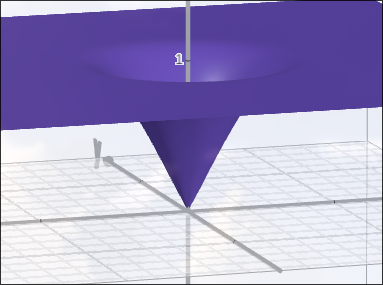
\includegraphics[width=0.3\linewidth]{chs/figs/sinkhole.png}
    \flushleft

    We see that when $ \vec p \neq \vec{0} $, then $ f $ is the composition of
    several continuous functions and is therefore continuous.
    At $ \vec{p} = \vec{0} $, we get that:
    \begin{align*}
        f(\vec{0}) & = \frac{2\alpha\left(\frac{1}{2}\right)}
        {\alpha\left( \frac{1}{2}\right)
        + \alpha\left( \frac{1}{2} \right)} - 1 \vsp
                   & = \frac{2\alpha \left( \frac{1}{2} \right)}
                   {2\alpha \left( \frac{1}{2} \right)} - 1 \vsp
                   & = 0
    \end{align*}
    So again by continuity of the composed functions, $ f $ is also continuous
    at $ 0 $. \vsp
    %
    (We'll drop the vector arrows from here on out.)
    To see that it is not totally differentiable at $ 0 $, suppose by
    contradiction it is. Then, there exists some $ L : \bb{R}^{2} \rightarrow
    \bb{R} $ such that:
    \begin{equation*}
        \lim_{h \rightarrow 0} \frac{\abs{f(0 + h) - f(0) - L(h)}} {\norm{h}}
        = \lim_{h \rightarrow 0} \frac{\abs{f(h) - L(h)}}{\norm{h}} = 0
    \end{equation*}
    By the reverse triangle inequality, we have that:
    \begin{align*}
        \frac{1}{\norm{h}}\abs{f(h) - L(h)} & \geq \frac{1}{\norm{h}}\abs{
        \abs{f(h)} - \abs{L(h)}} \vsp
        & \geq \frac{1}{\norm{h}}\abs{\abs{f(h)} + M\norm{h}} \vsp
        & = \abs{\frac{\abs{f(h)}}{\norm{h}} + M} \vsp
        & \geq \frac{\abs{f(h)}}{\norm{h}}
    \end{align*}
    So it suffices to show that as $ h \rightarrow 0,
    \dfrac{\abs{f(h)}}{\norm{h}} \cnot\rightarrow 0 $.
    Denote $ x = \norm{h} $ and $ y = \dfrac{2x}{1-x^{2}} $.
    Then, with some very extensive algebra, we have on $ [0, 1) $ that:
    \begin{align*}
        \frac{\abs{f(h)}}{x} & = \frac{1}{x} \cdot
        \frac{2e^{\frac{-2}{1+x}}}{e^{\frac{-2}{1+x}} + e^{\frac{-2}{1-x}}} - 1
        \vsp
        & = \frac{1}{x} \cdot \frac{e^{\frac{2}{1-x}}
        - e^{\frac{2}{1+x}}} {e^{\frac{2}{1-x}} + e^{\frac{2}{1+x}}} \vsp
        & = \frac{1}{x} \cdot \frac{e^{\frac{2(1+x)}{1-x^{2}}}
        - e^{\frac{2(1-x)}{1-x^{2}}}}
        {e^{\frac{2(1+x)}{1-x^{2}}} + e^{\frac{2(1-x)}{1-x^{2}}}} \vsp
        & = \frac{1}{x} \cdot \frac{e^{\frac{2+2x}{1-x^{2}}}
        - e^{\frac{2-2x}{1-x^{2}}}} {e^{\frac{2+2x}{1-x^{2}}}
        + e^{\frac{2-2x}{1-x^{2}}}} \vsp
        & = \frac{1}{x} \cdot \frac{e^{\frac{2}{1-x^{2}}}
        \left( e^{\frac{2x}{1-x^{2}}} - e^{\frac{-2x}{1-x^{2}}} \right)}
        {e^{\frac{2}{1-x^{2}}}\left( e^{\frac{2x}{1-x^{2}}}
        + e^{\frac{-2x}{1-x^{2}}} \right)} \vsp
        & = \frac{1}{x} \cdot \frac{e^{y} - e^{-y}}{e^{y} + e^{-y}} \vsp
        & = \frac{1}{x} \tanh(y) \vsp
        & = \frac{1}{x} \tanh \left( \frac{2x}{1-x^{2}} \right)
    \end{align*}
    We use L'Hopital's to see that the limit is given by:
    \begin{equation*}
        \lim_{x \rightarrow 0^{+}} \frac{1}{x}\tanh
        \left( \frac{2x}{1-x^{2}} \right)
        \ = \ \lim_{x \rightarrow 0^{+}} \sech^{2}
        \left( \frac{2x}{1-x^{2}} \right) \cdot
        \frac{2(1-x^{2}) + 4x}{(1-x^{2})^{2}}
    \end{equation*}
    The above is continuous on $ [0, 1) $, and expands to:
    \begin{equation*}
        \sech^{2}(y) \cdot \frac{2(1-x^{2}) + 4x}{(1-x^{2})^{2}}
        \ = \ \frac{4e^{2y}}{(e^{2y} +1)^{2}} \cdot \frac{2(1-x^{2}) + 4x}
        {(1-x^{2})^{2}}
    \end{equation*}
    At $ x = 0 $, we have that $ y = 0 $ as well. Putting it all together, we
    have that:
    \begin{equation*}
        \lim_{h\rightarrow0} \frac{\abs{f(h) - L(h)}}{\norm{h}}
        \ \geq \ \lim_{h\rightarrow0} \frac{\abs{f(h)}}{\norm{h}}
        \ = \ \frac{4 \cdot 1}{(1 + 1)^{2}} \cdot \frac{2(1) + 4 \cdot 0}
        {(1 - 0)^{2}} \ = \ 1 \cdot 2 \ = \ 2 \ \neq \ 0
    \end{equation*}
    We finally arrive at our contradiction, showing that $ f $ is not totally
    differentiable at the origin.
\end{pf} \vspace{-2mm}
The end of the proof suggests that this can be somewhat generalized to capture
``asymptotic" behaviour.
\begin{lm}[type=Conjecture.]
    Let $ U \subseteq \bb{R}^{n} $ be an open neighbourhood containing
    the origin. Given two continuous functions $ f, g : U \rightarrow \bb{R}^{m}
    $, suppose there exists a real number $ c > 0 $ satisfying the condition
    that: \vspace{-1mm}
    \begin{equation*}
        \lim_{x \rightarrow 0}\frac{\norm{f(x)}}{\norm{g(x)}} = c
    \end{equation*}
    Then $ f $ is differentiable at $ 0 $ if and only if $ g $ is differentiable
    at $ 0 $.
\end{lm}

\newpage
\subsubsection{Week 11 | Exercise 9.6}

The following is Exercise 9.6 from Week 11. This was solved and written
independently.

\begin{exr}[num=9.6]
    Let $ Q(x, y) = x^{2} + 5xy + 3y^{2} $. Find the corresponding symmetric
    matrix $ A $.
\end{exr}

\begin{pf}
    We know that $ A $ must be symmetric, so we can write:
    \begin{equation*}
        A = \begin{bmatrix}
            a & b \\ b & c
        \end{bmatrix}
    \end{equation*}
    where we solve for $ a, b, $ and $ c $.
    Note that:
    \begin{equation*}
        \vec{x}^{T}A\vec{x} \ = \
        \begin{bmatrix}
            x & y
        \end{bmatrix}
        \begin{bmatrix}
            a & b \\ b & c
        \end{bmatrix}
        \begin{bmatrix}
            x \\ y
        \end{bmatrix} \ = \
        ax^{2} + 2bxy + cy^{2}
    \end{equation*}
    Therefore, we set $ a = 1, b = \frac{5}{2}, $ and $ c = 3 $ to get the
    corresponding matrix. Note that this agrees with the derivation found in
    Exercise 9.5.
\end{pf}
\newpage
\subsubsection{Week 14 | Exercise 12.13}

The following is Exercise 12.13 from Week 14. This was solved and written
independently.
\vspace{-0.1in}
\begin{exr}[num=12.13]
    Let $ E \subseteq \bb{R}^{n} $ be a box. Let $ P, Q $ be partitions of $ E $
    such that $ Q $ refines $ P $ ($ P_{i} \subseteq Q_{i} $ for each $ i $).
    Show that $ U(f,P) \geq U(f,Q) $ and $ L(f,P) \leq L(f,Q) $.
\end{exr}
\vspace{-0.1in}
\begin{pf}
    Since $ P, Q $ both partition E, then:
    \begin{equation*}
        \sum_{j}\vol(P(j)) \ = \ \sum_{k}\vol(Q(k))
    \end{equation*}
    Furthermore, for any $ A \subseteq B \subseteq E $, we have that
    $ \trm{sup}_{A}(f) \leq \trm{sup}_{B}(f) $. Notice that for each $ Q(k) $,
    there exists a unique $ P(j) $ such that $ Q(k) \subseteq P(j) $. \vsp
    %
    Thus, reindex each $ Q(k) $ as $ Q(j, k_{j}) $, where $ j $ is the unique
    tuple such that $ Q(k) \subseteq P(j) $. Then, it follows that:
    \begin{align*}
        U(f, P) = \sum_{j}M_{j}\vol(P(j)) & \ = \sum_{j}M_{j} \left( \sum_{k_{j}}
        \vol(Q(j, k_{j})) \right) \\
                                          & \ = \sum_{j}\sum_{k}M_{j}
                                          \vol(Q(j,k_{j})) \\
                                          & \ \geq \sum_{j}\sum_{k}M_{k_{j}}
                                          \vol(Q(j,k_{j})) \\
                                          & \ = \sum_{k}M_{k}\vol(Q(k)) \\
                                          & \ = U(f, Q)
    \end{align*}
    Showing that $ L(f,P) \leq L(f, Q) $ is entirely analogous.
\end{pf}
\subsubsection{Week 16 | Exercise 14.10}

The following is Exercise 14.10 from Week 16.
This was solved together with Alan, and part of the write-up is done by Alan.

\begin{exr}[num=14.10a]
    Let $H$ be the open upper-hemisphere of the sphere in $\bb{R}^3$:
        \[ H = \{p=(x,y,z)\in S^3 :x^2+y^2+z^2=1, z>0\}. \]
        Find the surface area of $H$ using the parametrization
        $z=\sqrt{1-x^2-y^2}$.
\end{exr}

\begin{pf}
    Denote our parametrization $ f: B_{2}(0, 1) \rightarrow H $ as:
    \begin{equation*}
        f(x, y) = (x, y, \sqrt{1 - x^{2} - y^{2}})
    \end{equation*}
    We want to compute the following:
    \begin{equation*}
        \trm{vol}_{f}(H) = \int_{B_{2}(0, 1)}V(Jf)
        = \int_{B_{2}(0, 1)}\sqrt{\det\left((Jf)^{\msf{T}}(Jf)\right)}
    \end{equation*}
    Note that $ B_{2}(0, 1) $ simply denotes the unit ball in $ \bb{R}^{2} $.
    We calculate the Jacobian of $ f $ as:
    \begin{equation*}
        Jf =
        \begin{bmatrix}
            1 & 0 \\
            0 & 1 \\
            \dfrac{-x}{\sqrt{1-x^{2}-y^{2}}} & \dfrac{-y}{\sqrt{1-x^{2}-y^{2}}}
        \end{bmatrix}
    \end{equation*}
    Then, we see that:
    \begin{align*}
        (Jf)^{\msf{T}}Jf & \ = \
        \begin{bmatrix}
            1 & 0 & \dfrac{-x}{\sqrt{1-x^{2}-y^{2}}} \\[0.15in]
            0 & 1 & \dfrac{-y}{\sqrt{1-x^{2}-y^{2}}}
        \end{bmatrix}
        \begin{bmatrix}
            1 & 0 \vsp
            0 & 1 \vsp
            \dfrac{-x}{\sqrt{1-x^{2}-y^{2}}} & \dfrac{-y}{\sqrt{1-x^{2}-y^{2}}}
        \end{bmatrix} \vsp
                         & \ = \
        \begin{bmatrix}
            1 + \dfrac{x^{2}}{1-x^{2}-y^{2}} & \dfrac{xy}{1-x^{2}-y^{2}}
            \\[0.15in]
            \dfrac{xy}{1-x^{2}-y^{2}} & 1+\dfrac{y^{2}}{1-x^{2}-y^{2}}
        \end{bmatrix}
    \end{align*}
    The determinant is thus given as:
    \begin{align*}
        \det \left( (Jf)^{\msf{T}}(Jf) \right) & \ = \
        \left( 1 + \frac{x^{2}}{1-x^{2}-y^{2}} \right)
        \left( 1 + \frac{y^{2}}{1-x^{2}-y^{2}} \right) -
        \left( \frac{xy}{1-x^{2}-y^{2}} \right)^{2} \vsp
        & \ = \
        1 + \frac{x^{2}}{1-x^{2}-y^{2}} + \frac{y^{2}}{1-x^{2}-y^{2}} \vsp
        & \ + \ \left( \frac{xy}{1-x^{2}-y^{2}} \right)^{2} -
        \left( \frac{xy}{1-x^{2}-y^{2}} \right)^{2} \vsp
        & \ = \
        \frac{1-x^{2}-y^{2}}{1-x^{2}-y^{2}} +
        \frac{x^{2}}{1-x^{2}-y^{2}} + \frac{y^{2}}{1-x^{2}-y^{2}} \vsp
        & \ = \ \frac{1}{1-x^{2}-y^{2}} \vsp
        \trm{vol}_{f}(H) & \ = \ \int_{B_{2}(0,1)}
        \sqrt{\det \left( Jf \right)^{\msf{T}}Jf} \\
                         & \ = \ 4\int_{0}^{1}\int_{0}^{\sqrt{1-x^{2}}}
                         \sqrt{\frac{1}{1-x^{2}-y^{2}}}\d y\d x \\
                         & \ = \ 4\int_{0}^{1}\int_{0}^{\sqrt{1-x^{2}}}
                         \frac{1}{\sqrt{1-x^{2}-y^{2}}}\d y\d x \vsp
                         & \ = \ 4\int_{0}^{1}\arcsin \left(
                             \frac{y}{\sqrt{1-x^{2}}}
                         \right)\bigg\rvert_{0}^{\sqrt{1-x^{2}}}\d x
                         \tag*{(thx Alan)}\vsp
                         & \ = \ 4\int_{0}^{1} \frac{\pi}{2}\d x \vsp
                         & \ = \ 2\pi
    \end{align*}
    Therefore, we conclude that $ \trm{vol}_{f}(H) = 2\pi $ as needed.
\end{pf}

\begin{exr}[num=14.10b]
    Find the surface area of $H$ using spherical coordinates.
\end{exr}

\begin{pf}[source=Alan]
    Let $\alpha : (0, 2\pi) \times (0, \frac{\pi}{2}) \rightarrow H$ be a
    parametrization of $H$ using spherical coordinates where:
$$
\alpha(\theta, \phi) = (\sin(\phi)\cos(\theta), \sin(\phi)\sin(\theta),
\cos(\phi))
$$

Then we wish to compute:
$$
\operatorname{vol}_\alpha(H) = \int_{(0, 2\pi) \times (0, \frac{\pi}{2})}
V(\alpha^\prime)
$$

First, observe that:
\begin{gather*}
\alpha^\prime(\theta, \phi) = \begin{bmatrix}
-\sin(\phi)\sin(\theta) & \cos(\phi)\cos(\theta) \\
\sin(\phi)\cos(\theta) & \cos(\phi)\sin(\theta) \\
0 & -\sin(\phi)
\end{bmatrix} \vsp
\alpha^\prime(\theta, \phi)^T = \begin{bmatrix}
-\sin(\phi)\sin(\theta) & \sin(\phi)\cos(\theta) & 0 \\
\cos(\phi)\cos(\theta)  & \cos(\phi)\sin(\theta) & -\sin(\phi)
\end{bmatrix}
\end{gather*}

For brevity, we'll denote $ \omega(\phi, \theta) = \sin(\phi)\sin(\theta) $
and $ \tau(\phi, \theta) = \cos(\phi)\cos(\theta) $.
Then, observe that:
\begin{align*}
    & (\alpha^\prime(\theta, \phi))^t\alpha^\prime(\theta, \phi) \\ = &
\begin{bmatrix}
\omega^{2}(\phi, \theta) + \sin^2(\phi)\cos^2(\theta) & -\omega(\phi, \theta)
\tau(\phi, \theta)
+ \tau(\phi, \theta)\omega(\phi, \theta) \\ 
-\omega(\phi, \theta)\tau(\phi, \theta) + \tau(\phi, \theta)\omega(\phi,\theta) &
\tau^{2}(\phi, \theta) + \cos^2(\phi)\sin^2(\theta) + \sin^2(\phi) \\
\end{bmatrix} \vsp
    = & 
\begin{bmatrix}
\omega^{2}(\phi, \theta) + \sin^2(\phi)\cos^2(\theta) & 0 \\ 
0 & \tau^{2}(\phi, \theta) + \cos^2(\phi)\sin^2(\theta) + \sin^2(\phi) \\
\end{bmatrix}
\end{align*}

Finally, we have that $ \det(\alpha^\prime(\theta, \phi))^t\alpha^\prime
(\theta, \phi)) $
is given by:
\begin{align*}
    & \ (\omega^{2}(\phi, \theta) + \sin^{2}(\phi)\cos^{2}(\theta))
    (\tau^{2}(\phi, \theta)+\cos^{2}(\phi)\sin^{2}(\theta)+\sin^{2}(\phi)) \\
= & \ (\sin^2(\phi)\sin^2(\theta) + \sin^2(\phi)\cos^2(\theta))(\cos^2(\phi)
\cos^2(\theta) +
\cos^2(\phi)\sin^2(\theta) + \sin^2(\phi)) \\
 = & \ (\sin^2(\phi)(\sin^2(\theta) + \cos^2(\theta)))(\cos^2(\phi)
 (\cos^2(\theta) + \sin^2(\theta))
 + \sin^2(\phi)) \\
 = & \ (\sin^2(\phi))(\cos^2(\phi) + \sin^2(\phi)) \\
 = & \ \sin^2(\phi) \\
\end{align*}

As a result:
\begin{align*}
\operatorname{vol}_\alpha(H) &= \int_{(0, 2\pi) \times (0, \frac{\pi}{2})}
V(\alpha^\prime) \\
 &= \int_{(0, 2\pi) \times (0, \frac{\pi}{2})} \sqrt{ \det (\alpha^\prime)^t
 (\alpha^\prime)  } \\
 &= \int_{0}^{2\pi} \int_0^{\frac{\pi}{2}} \sqrt{ \sin^2(\phi)  }   d\phi d\theta
 \\
 &= \int_{0}^{2\pi} \int_0^{\frac{\pi}{2}} \sin(\phi)  d\phi d\theta \quad \left(
     \sin \text{ is
 positive on } \left[0, \frac{\pi}{2}\right]\right) \\
 &= \int_{0}^{2\pi} \int_0^{\frac{\pi}{2}} \sin(\phi)  d\phi d\theta \\
 &= \int_{0}^{2\pi} -\cos(\frac{\pi}{2}) + \cos(0)  d\theta \\
 &= \int_{0}^{2\pi} 1  d\theta \\
 &= 2\pi \\
\end{align*}
\end{pf}

\newpage
\subsubsection{Week 18 | Exercise 17.4}

The following is Exercise 17.4 from Week 18. This was solved and written
independently.

\begin{exr}[num=17.4]
    Show that $ S^{2} $ is orientable.
\end{exr}

\begin{pf}
    Showing that $ S^{2} $ is orientable can be done trivially using spherical
    coordinates, as transition maps are simply the identity. Thus, we will opt
    for a different atlas. \vsp
    %
    Denote by $ S_{1} $ the set $ S^{2} \setminus \set{(0, 0, 1)} $. Similarly
    denote by $ S_{2} $ the set $ S^{2} \setminus \set{(0, 0, -1)} $. We have
    charts given by stereographic projections:
    \begin{gather*}
        \vphi_{1}(x, y) \ = \ \left( \frac{2x}{1+x^{2}+y^{2}},
        \frac{2y}{1+x^{2}+y^{2}},\frac{x^{2}+y^{2}-1}{1+x^{2}+y^{2}}\right) \vsp
        \vphi_{2}^{-1}(a,b,c) \ = \ \left( \frac{-a}{1+c}, \frac{b}{1+c} \right)
    \end{gather*}
    Then $ \vphi = \vphi_{2}^{-1}\circ\vphi_{1}:\vphi_{1}^{-1}(S_{1}\cap S_{2})
    \gto \vphi_{2}^{-1}(S_{1}\cap S_{2}) $ is a diffeomorphism. To see that it
    is orientation-preserving, we take the determinant of the Jacobian:
    \begin{gather*}
        \vphi_{2}^{-1}\circ\vphi_{1}(x,y) \ = \
        \left(\frac{-x}{x^{2}+y^{2}}, \frac{y}{x^{2}+y^{2}}\right) \vsp
        J\vphi \ = \
        \begin{bmatrix}
            \dfrac{x^{2}-y^{2}}{(x^{2}+y^{2})^{2}} &
            \dfrac{2xy}{(x^{2}+y^{2})^{2}} \\[1.5em]
            \dfrac{-2xy}{(x^{2}+y^{2})^{2}} &
            \dfrac{x^{2}-y^{2}}{(x^{2}+y^{2})^{2}}
        \end{bmatrix} \\[1em]
        \det(J\vphi) \ = \ \frac{(x^{2}-y^{2})^{2}+4x^{2}y^{2}}
        {(x^{2}+y^{2})^{4}} \ = \ \frac{1}{(x^{2}+y^{2})^{2}}
    \end{gather*}
    Note that $ x = y = 0 $ is not in the domain, as the charts do not intersect
    on either pole. Thus, it is clearly always positive, and so $ S^{2} $ is
    indeed orientable.
\end{pf}
Conjecture: it is not possible to orient $ S^{2} $ using the six natural
hemispheres and standard Cartesian coordinates as charts.

Intuitively: the six hemispheres induce three circle ``axes"; these cannot be
oriented consistently using only two axes in $ \bR^{2} $.

\newpage
\subsubsection{Week 19 | Exercise 18.18}

The following is Exercise 18.18 from Week 19. This was solved and written
independently.

\begin{exr}[num=18.18]
    Does closed imply conservative?
\end{exr}

\begin{pf}
    No. Consider the field $ F $ given by:
    \begin{equation*}
        F(x, y) \ = \ \frac{-y}{x^{2}+y^{2}}, \frac{x}{x^{2}+y^{2}}
    \end{equation*}
    To see that this is closed, notice:
    \begin{gather*}
        \frac{\p F_{1}}{\p y} \ = \ \frac{-(x^{2}+y^{2})+2y^{2}}
        {(x^{2}+y^{2})^{2}} \ = \ \frac{y^{2}-x^{2}}{(x^{2}+y^{2})^{2}} \vsp
        \frac{\p F_{2}}{\p x} \ = \ \frac{(x^{2}+y^{2})-2x^{2}}
        {(x^{2}+y^{2})^{2}} \ = \ \frac{y^{2}-x^{2}}{(x^{2}+y^{2})^{2}}
    \end{gather*}
    To see that $ F $ is not conservative, consider $ \gamma:[0, 2\pi]\gto
    S^{1} $ where $ \gamma(\theta) = (\cos\theta, \sin\theta) $. Then:
    \begin{equation*}
        \oint_{C}F\cdot\di x \ = \ \int^{2\pi}_{0}F(\gamma(t))\cdot
        \gamma'(t)\di t
    \end{equation*}
    Notice:
    \begin{gather*}
        F(\gamma(t)) \ = \ (-\sin\theta, \cos\theta) \\
        \gamma'(t) \ = \
        \begin{bmatrix}
            -\sin\theta & \cos\theta
        \end{bmatrix}^{T} \\
        F(\gamma(t))\cdot\gamma'(t) \ = \ 1
    \end{gather*}
    Thus, we have that:
    \begin{equation*}
        \oint_{C}F\cdot\di x \ = \
        \int_{0}^{2\pi}F(\gamma(t))\cdot\gamma'(t)\di t \ = \
        \int_{0}^{2\pi}1\di t \ = \ 2\pi
    \end{equation*}
    Thus $ F $ is not conservative.
\end{pf}
